\documentclass[12pt,a4paper]{report}
\usepackage[utf8]{inputenc} % this is needed for umlauts
\usepackage[ngerman]{babel} % this is needed for umlauts
\usepackage[T1]{fontenc}    % this is needed for correct output of umlauts in pdf

\usepackage{ucs}
\usepackage{amsmath}
\usepackage{amsfonts}
\usepackage{amssymb}
\usepackage{graphicx}

\usepackage{hyperref}
\usepackage{csquotes}
\usepackage{appendix}
\usepackage{pdfpages}

\begin{document}

	\tableofcontents
	\newpage
	
	\chapter{Vorwort}
	Dieses Dokument findest du auf github.com unter: \href{https://github.com/henri-libre/analysis1}{https://github.com/henri-libre/analysis1}. Du darfst das Dokument nutzen, erweitern und verbreiten. Maintainer des Dokumentes erreichst du entweder dort oder per E-Mail an \href{analysis1istgeil@nanooq.org}{analysis1istgeil@nanooq.org}. Für die Korrektheit des Dokumentes ist entweder keiner oder du verantwortlich. Die URL der Veranstaltung an sich lautet: \href{https://analysis3.wordpress.com/analysis-i-ws-1516/uebungen-zu-analysis-i-wise-1516/}{https://analysis3.wordpress.com/analysis-i-ws-1516/uebungen-zu-analysis-i-wise-1516/}
	
\chapter{Übungsblatt 1}
	
	Das entsprechende Übungsblatt befindet sich im Anhang \ref{uebungsblatt1}.
	
	\section{Aufgabe 1:}
	Beweisen Sie mit vollständiger Induktion: Für alle $ n \in N $ gilt:
	\begin{enumerate}
	\item $ 5^n - 1 $ ist durch 4 teilbar.
	\item $ 3^{2^n} - 1 $ ist durch $ 2^(n+2)$ teilbar.
	\item Die Anzahl $A_n$ aller Teilmengen einer $n$-elementigen Menge ist gegeben durch $A_n=2^n$
	\end{enumerate}
	
	\subsection{Musterlösung}
	Noch nicht bekannt gegeben
	
	\subsection{Lösung Lerngruppe \enquote{HenriLibre, du?, du?, du?}}
	\begin{enumerate}
	\item z.~z.: $5^n - 1 | 4 $ 
		\begin{itemize}
			\item Induktionsanker:\\
			$n_1 = 1: 5^1 - 1 = x \cdot 4$ \\
			$\Leftrightarrow 5-1 = x \cdot 4 $ \\
			$\Leftrightarrow x = 4 $ \\
			\item Induktionsvoraussetzung:\\
			$ (5^n -1)$ ist durch 4 teilbar.\\
			\item Induktionsschritt: \\ 
			$ n \mapsto n+1: a_{n+1} = 5^{n+1}-1$ \\ 
			$ = (5 \cdot 5^n)-1$ \\
			$ (4 \cdot 5^n + 5^n) -1$ \\
			$ (4 \cdot 5^n) + (5^n -1)$\\
			Erster Term ist per Definition durch 4 teilbar. Zweiter Term ist gleich unserer Induktionsvoraussetzung.  
		\end{itemize}
	\item z.~z.: $ 3^{2^n}-1|2^{n+2} $ 
		\begin{itemize}
			\item Induktionsanker:\\
			$ n_1 = 1: 3^2 -1 = 9 - 1 = 8 $
			\item Induktionsvoraussetzung:\\
			$ 3^{2^n} - 1 $ durch $ 2^{n+2} $ teilbar.
			\item Induktionsschritt: \\ 
			$ n \mapsto n+1: 3^{2^{n+1}} -1 \\
			\overset{\text{aus der Kla-}}{\underset{\text{mer ziehen}}{=}} (3^{2^n})^2 -1\\ \overset{\text{Binomische}}{\underset{\text{Formel}}{=}} (3^{2^n}-1)(3^{2^n}+1)$ \\
			Erster Term ist die Induktionsvoraussetzung. Der zweite Term ist im Detail unwichtig, wegen der Multiplikation.
		\end{itemize}
	\item z.~z.: Für Menge $M$ mit $|M| = n \Rightarrow |P(M)|=2^n$
		\begin{itemize}
			\item Induktionsvoraussetzung:\\
			$ n=1: $ Sei $M=\{n\}$. Dann ist $P(M)=\{\varnothing,\{a\}\} \rightarrow |P(M)|=2^1$.
			\item Induktionsschritt:\\
			Dann sei $M^*=\{a_1,\dots, a_n\}$.\\
			Dann gilt laut Induktionsvoraussetzung: $|P(M^*)=2^n|$.
			\\Nun gilt\footnote{$P(M) \setminus P(M^*)$ muss disjunkt sein, weil: Wenn A, B disjunkt, dann $ A \cap B = \varnothing$.} $P(M) \setminus P(M^*) = \{T \cup \{a_{n+1}\} | T \in P(M^*)\} \\
			\Rightarrow |P(M)|=2|P(M^*)|=2\cdot 2^n= 2^{n+1}$
			\item Erklärung:\\
			Es sei $ P(m^*) = \{\varnothing\}, \{a_1\}, \{a_2\}, \{a_1,a_2\}$. Wenn nun $ \{a_3\} $ hinzugefügt wird, ist $ P(m) = P(m^*) \cup \{a_{3}\} = \{\varnothing\}, \{a_1\}, \{a_2\}, \{a_1,a_2\},\\
			\{a_3\}, \{a_1,a_3\}, \{a_2,a_3\}, \{a_1,a_2,a_3\} $.
		\end{itemize}
	\end{enumerate}

\appendices
	\chapter{}
	\section{Übungsblatt 1}\label{uebungsblatt1}
	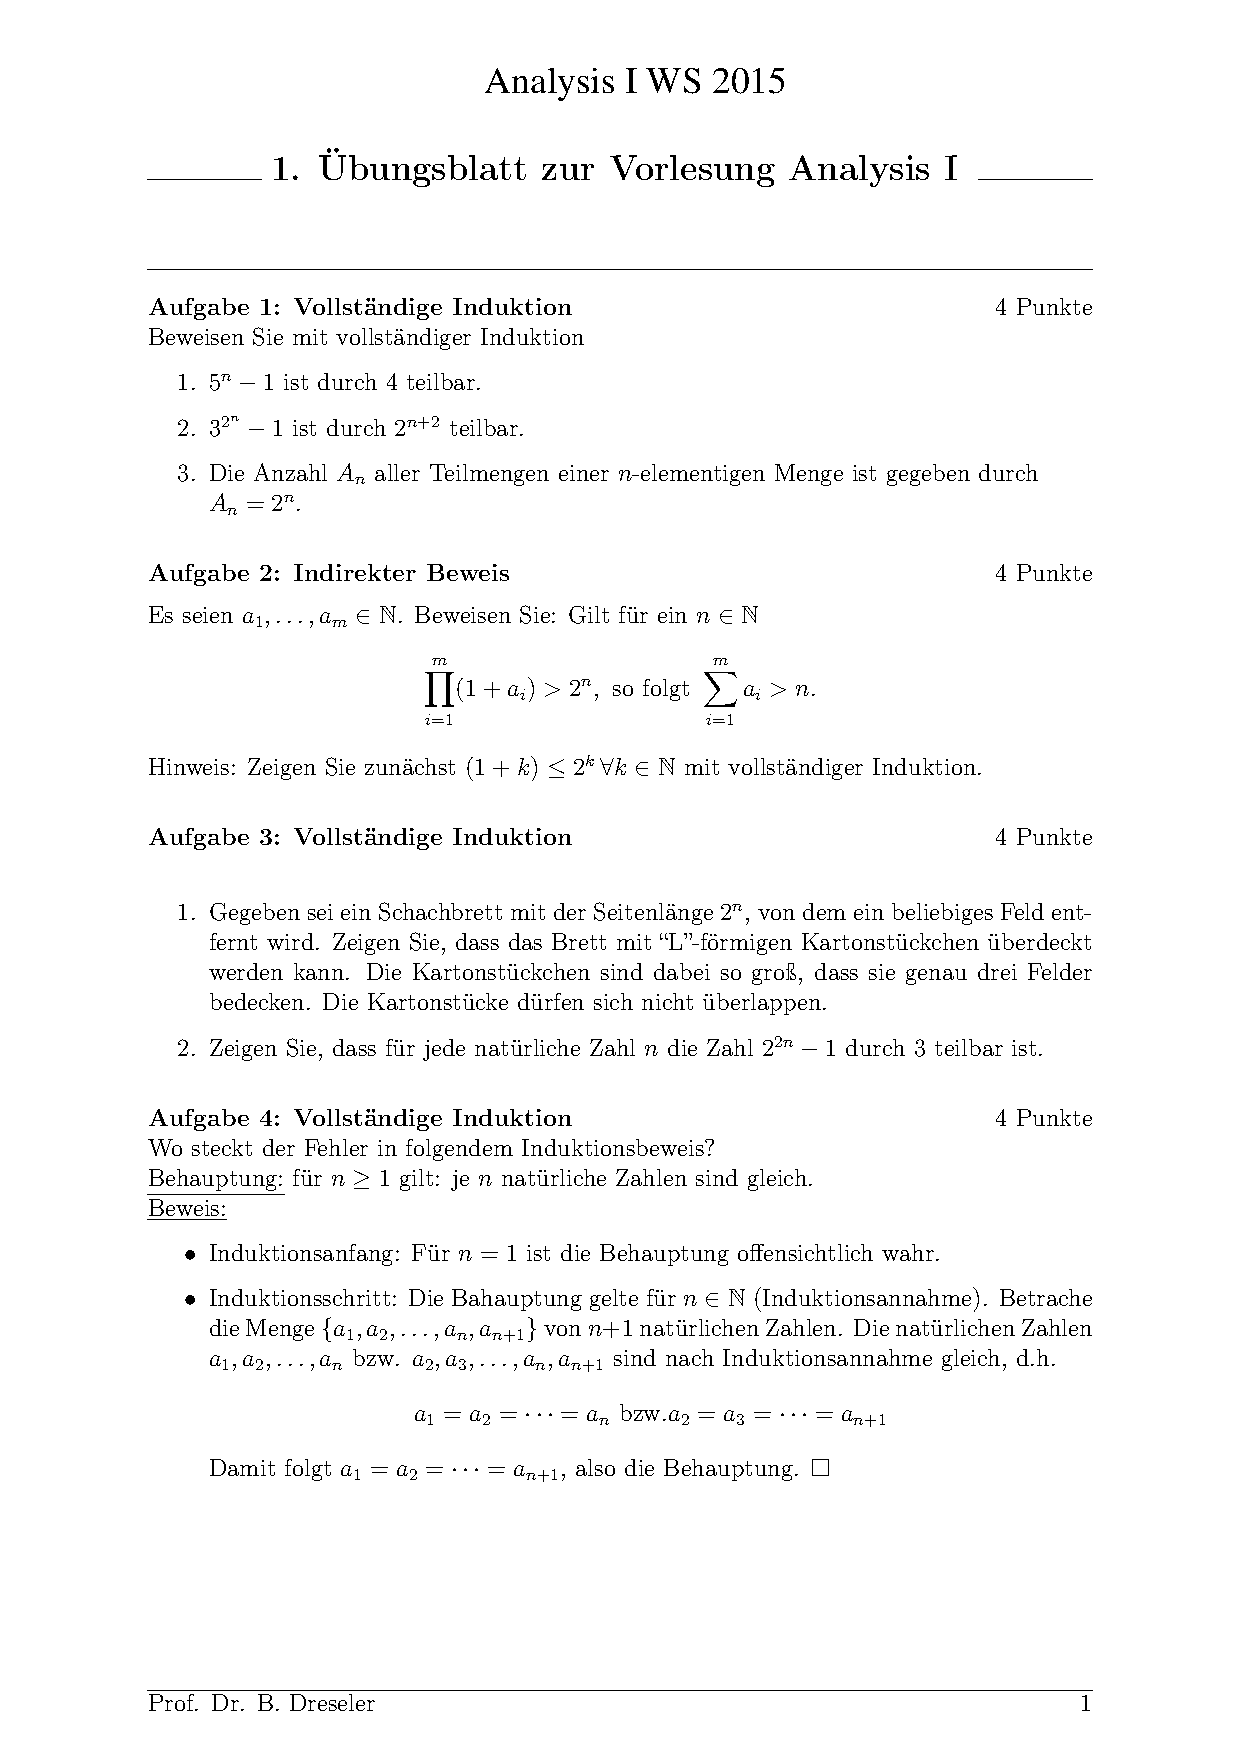
\includepdf[pages=-]{blatt1}
\end{document}